\chapter{Common-Emitter BJT Amplifier}


\section{Objectives}
\begin{itemize}
    \item To measure the quiescent-point of a common-emitter BJT amplifier
    \item To evaluate the small-signal amplification function of a common-emitter amplifier
\end{itemize}

\section{Materials}
\begin{itemize}
    \item \hyperref[2N3904_1]{BJT (2N3904)}
    \item Breadboard
    \item Capacitors
    \item DC power supply
    \item Digital Multi-Meter
    \item Function Generator
    \item Oscilloscope
    \item Resistors
\end{itemize}

\section{Introduction}
    \subsection{Circuit Diagram}
    \begin{figure}[h]
        \centering
        \includesvg[width=0.7\linewidth]{Lab06/Lab6.drawio.svg}
        \caption{A common-emitter amplifier}
        \label{lab6f}
    \end{figure}
    \FloatBarrier
In Fig.\ref{lab6f}, $V_{BEQ}$ = 0.65 V, $\beta$ = 160, $R_s$ = 2k$\Omega$, $R_a$ = 56k$\Omega$, $R_b$ = 27$\Omega$, $R_C$ = 1k$\Omega$, $R_E$ = 2k$\Omega$.

\section{Detailed Procedures}
    \subsection{Analyzation}
    First, we analyze the circuit by drawing its AC-equivalent and DC-equivalent circuit.\par
    \begin{itemize}
        \item AC-equivalent Circuit:\par
            \begin{figure}[h]
                \centering
                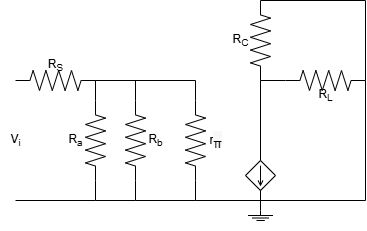
\includegraphics[width=0.6\linewidth]{Lab06/Lab6ac.drawio.png}
                \caption{AC-equivalent Circuit}
                \label{l6ac}
            \end{figure}
            \FloatBarrier
        \item DC-equivalent Circuit:\par
            \begin{figure}[h]
                \centering
                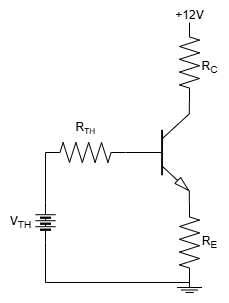
\includegraphics[width=0.4\linewidth]{Lab06/Lab6dc.drawio.png}
                \caption{DC-equivalent Circuit}
                \label{l6dc}
            \end{figure}
            \FloatBarrier
    \end{itemize}
    In Fig.\ref{l6ac}\par
    \begin{equation}
            r_\pi=\frac{V_{be}}{i_b}
    \end{equation}
    
    In Fig.\ref{l6dc}\par
    \begin{equation}
        \begin{cases}
            R_{TH} = R_a//R_b\\
            V_{TH} = 12\cdot\frac{R_b}{R_a//R_b}\\
            12-i_cR_c-V_{CE}-i_ER_E=0\\
            V_{TH}-i_bR_{TH}-V_{BE}-i_eR_E=0\\
        \end{cases}
    \label{l6eq1}
    \end{equation}
    From Equation.\ref{l6eq1} and given data, we can obtain:\par
    \begin{equation*}
        \begin{cases}
            i_b = 9.56\mu A\\
            i_c = 1.53296 mA\\
            i_e = 1.53916 mA\\
            V_B = 3.903 V\\
            V_C = 10.47 V\\
            V_E = 3 V\\
            V_{CE} = 7.4 V
        \end{cases}
    \end{equation*}

    \subsection{Procedures}
    \begin{itemize}
    \item DC Analysis\par
    \begin{table}[h]
    \centering
        \begin{tabular}{|c|c|c|c|c|c|c|c|}
        \hline
        & $V_B$ & $V_C$  & $V_E$ & $I_B$ & $I_C$  & $I_E$  & $\beta$ \\ \hline
        Meas & 3.776 & 10.435 & 3.118 & 12.3u & 1.565m & 1.553m & 127     \\ \hline
        Theo & 3.903 & 10.47  & 3     & 9.56u & 1.533m & 1.539m & 160     \\ \hline
    \end{tabular}
    \end{table}
    \FloatBarrier
    
    \item AC Analysis: Voltage Gain\\
    ($V^*$ that does not distort output voltage = 0.020 V)\par
    \begin{table}[h]
    \centering
        \begin{tabular}{|c|c|c|c|c|}
        \hline
        $v_{ib}$ & 5.5  & 8.25 & 11   & 13.4 \\ \hline
        $v_o$    & 212  & 317  & 422  & 605  \\ \hline
        $A_v$    & 38.5 & 38.4 & 38.4 & 45.1 \\ \hline
    \end{tabular}
    \end{table}
    \FloatBarrier
    We took $V^* = 0.25V$, which is the voltage not distorting output.
    \FloatBarrier
    \begin{figure}[h]
        \centering
        \includegraphics[width=0.5\linewidth]{Lab06/Images/6.6_Vi-Vib_a.jpg}
        \caption{1000Hz, 0.5V peak}
        \label{l6acvg}
    \end{figure}
    \FloatBarrier
    \begin{figure}[h]
        \centering
        \includegraphics[width=0.5\linewidth]{Lab06/Images/6.5_Vo-Vib_distrupted.jpg}
        \caption{Disrupted Waveform}
        \label{l6dcdisrupted}
    \end{figure}
    \FloatBarrier
    \begin{figure}[h]
        \centering
        \includegraphics[width=0.5\linewidth]{Lab06/Images/6.5_Vo-Vib_025mV.jpg}
        \caption{0.025V Waveform}
        \label{l6dc025}
    \end{figure}
    \FloatBarrier
    \begin{figure}
        \centering
        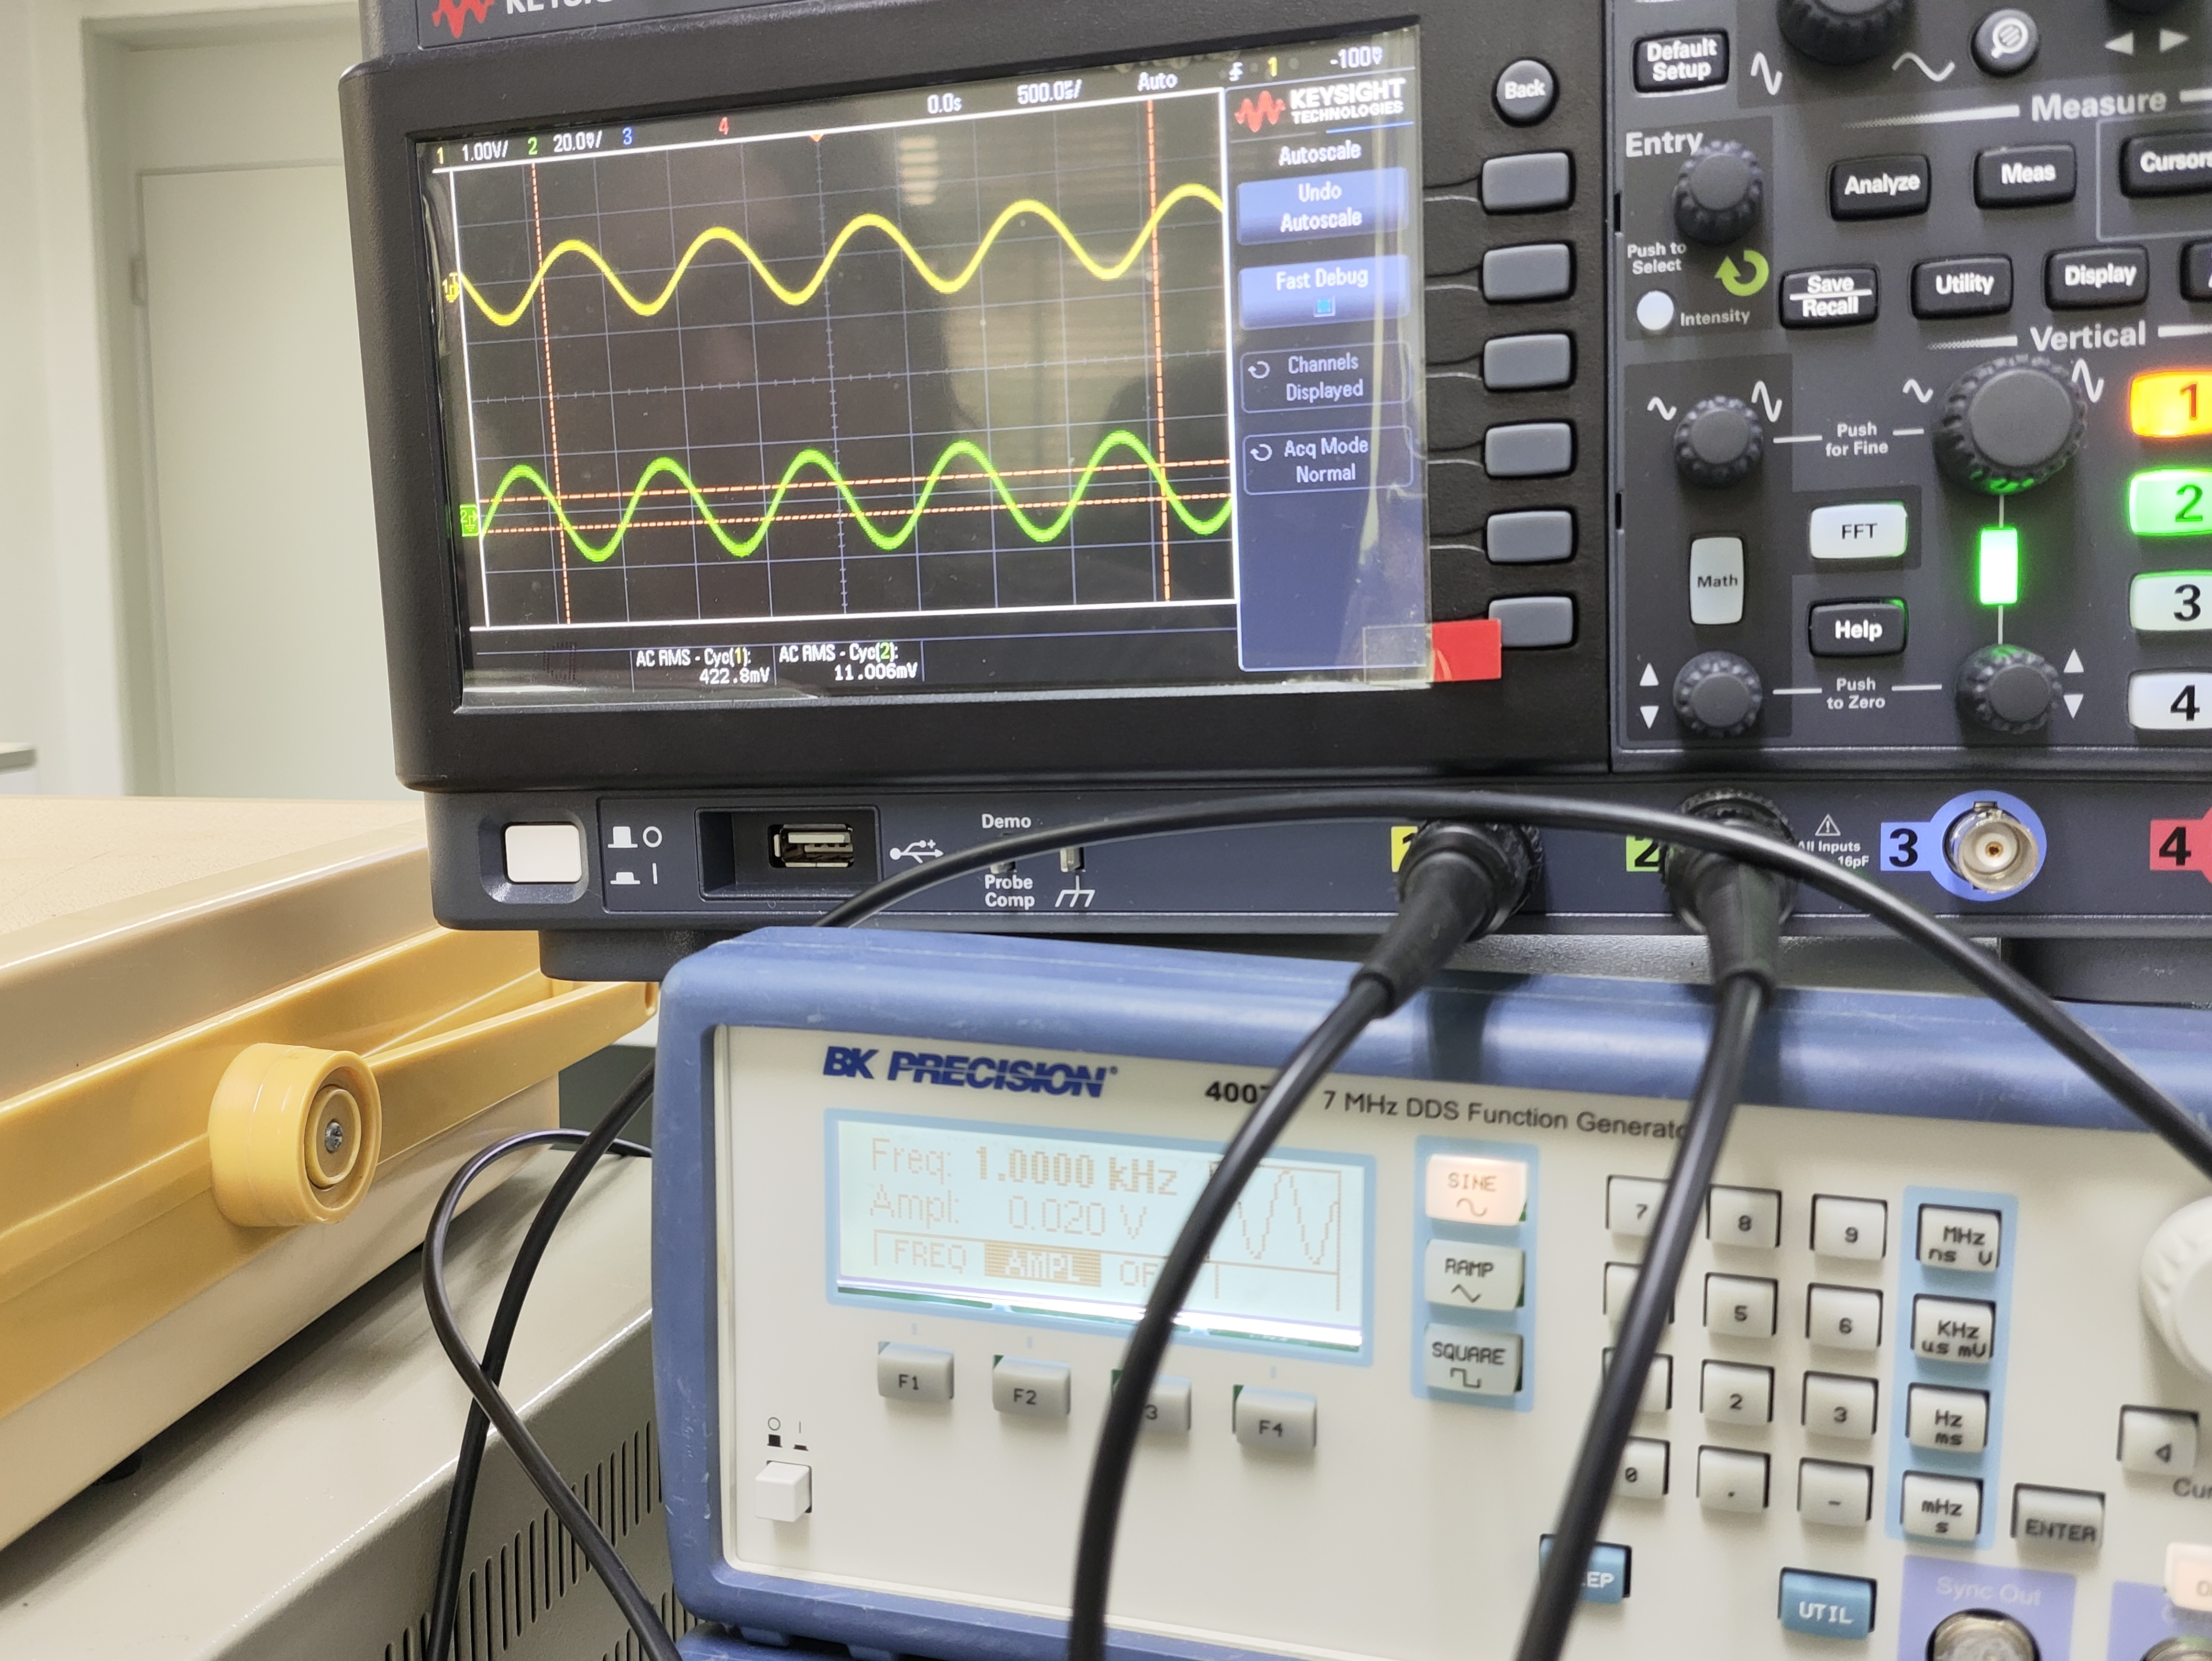
\includegraphics[width=0.5\linewidth]{Lab06/Images/6.5_Vo-Vib_020mV.jpg}
        \caption{0.020V Waveform}
        \label{l6dc020}
    \end{figure}
    \FloatBarrier
    \begin{figure}
        \centering
        \includegraphics[width=0.5\linewidth]{Lab06/Images/6.5_Vo-Vib_015mV.jpg}
        \caption{0.015V Waveform}
        \label{l6acvg015}
    \end{figure}
    \FloatBarrier
    \begin{figure}[h]
        \centering
        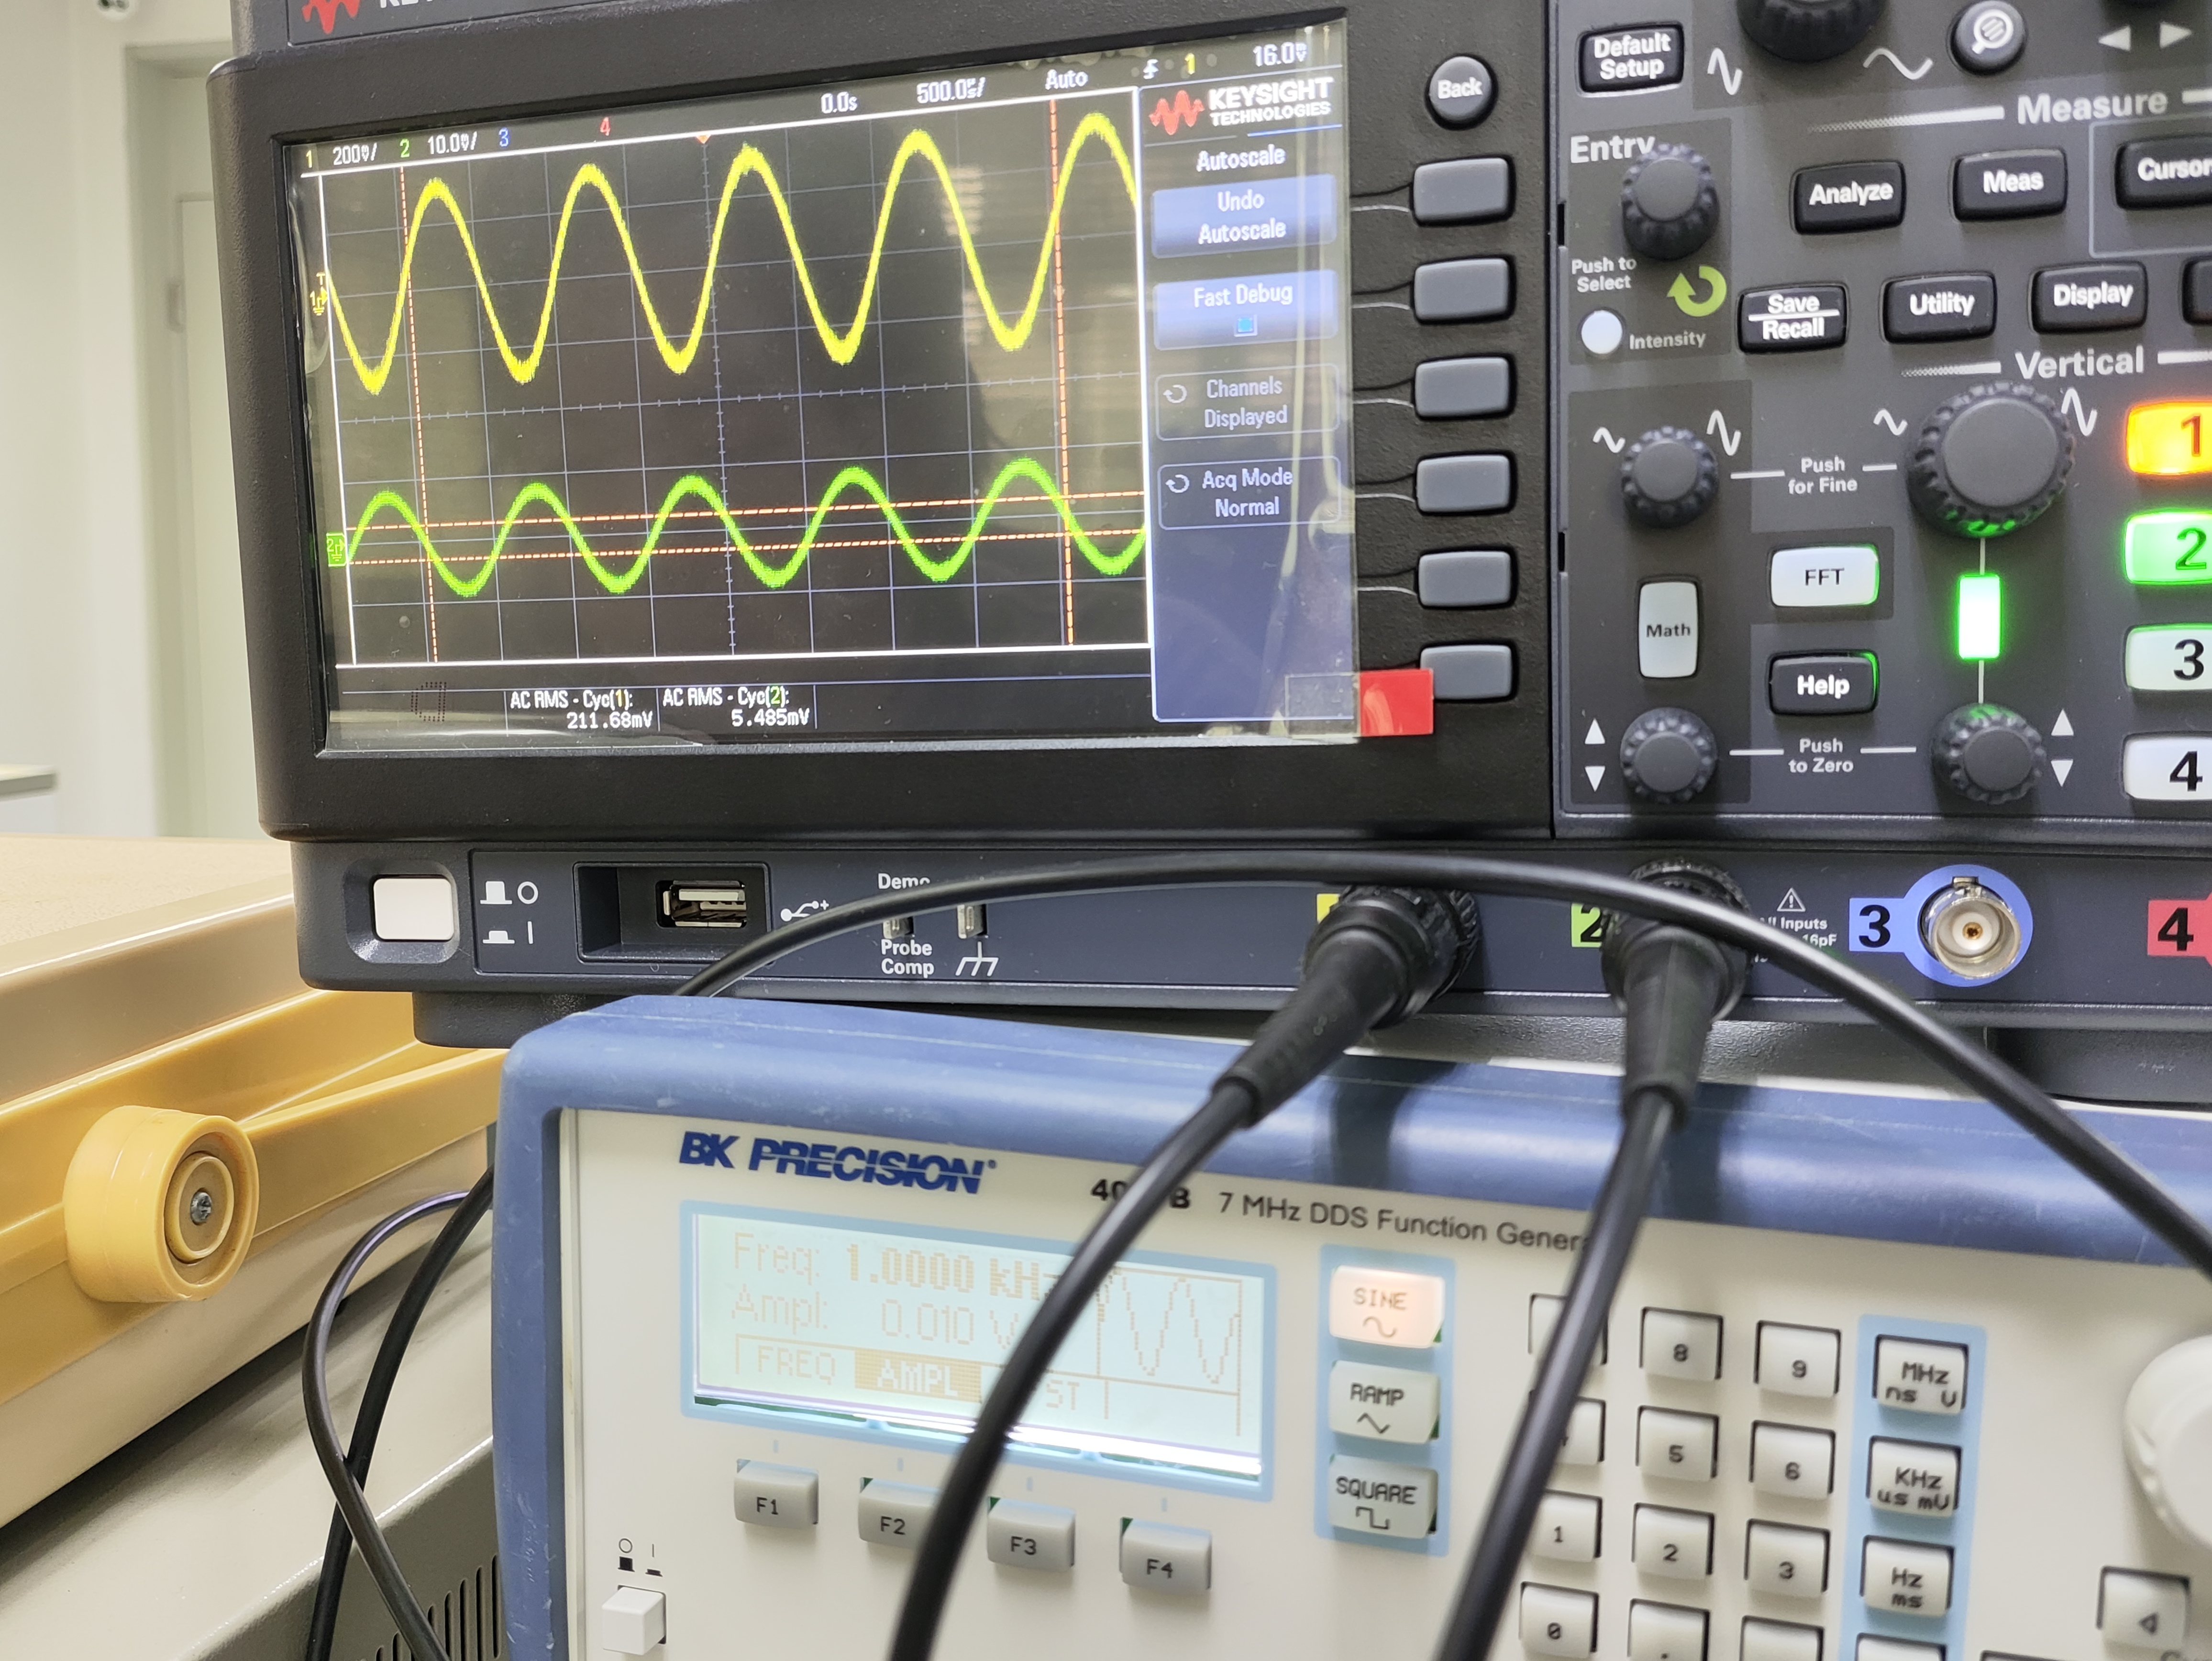
\includegraphics[width=0.5\linewidth]{Lab06/Images/6.5_Vo-Vib_010mV.jpg}
        \caption{0.10V Waveform}
        \label{l6acvg010}
    \end{figure}
    \FloatBarrier
    {\small *Due to the limitation of the Function Generator, we were unable to vary $V^*$ to 20\%.}\par
    When the distortion emerges, it is into the saturation mode, $R_a$ should be increased.
    \FloatBarrier
    \item AC Analysis: Resistance\\
    ($V^*$ = 0.025 V for Input, $V^*$ = 0.160 V for Output)\par
    \begin{table}[h]
    \centering
        \begin{tabular}{|cc|cc|}
        \hline
        \multicolumn{2}{|c|}{$R_s=2k,~R_i=13.55k$}               & \multicolumn{2}{c|}{$R_o=R_C//R_L$}                                   \\ \hline
        \multicolumn{1}{|c|}{$v_i=18.1m$} & $V_{ib}=13.7m$ & \multicolumn{1}{c|}{$R_L=300K,~V_o=219$} & $R_L=2K,~V_o=393$ \\ \hline
        \multicolumn{1}{|c|}{$v_i=10.8m$} & $V_{ib}=8.2m$  & \multicolumn{1}{c|}{}                    &                   \\ \hline
        \multicolumn{1}{|c|}{$v_i=7.24m$} & $V_{ib}=5.48m$ & \multicolumn{1}{c|}{}                    &                   \\ \hline
    \end{tabular}
    \end{table}
    \FloatBarrier
    \end{itemize}
    \FloatBarrier
\section{Discussion}
The theoretical values and measured values are different in real life, $V_{BE}$ and resistors may not be ideal as expected.\par
Furthermore, we take the ideal data in calculation, with more and more steps during calculating, the errors will be enlarged.

\section{Conclusion}
In conclusion, we learned more about basic principle of a common-emitter BJT amplifier after conducting this experiment.\par
The CE amplifier provides significant voltage gain, making it suitable for signal amplification in electronic circuits. Additionally, the phase shift of 180-degree is observed between the input and output signals, it is the characteristic of the common-emitter configuration.\par
Overall, this experiment helps us to understand the design and practical considerations of BJT amplifiers.